%Adaptado de
%=========
%% bare_jrnl.tex
%% V1.4b
%% 2015/08/26
%% by Michael Shell
%=======
%Definición del tipo de documento
\documentclass[journal]{IEEEtran}
%Paquetes que se usarán
%Adaptado de
%=========
%% bare_jrnl.tex
%% V1.4b
%% 2015/08/26
%% by Michael Shell
%=======
%Definición del tipo de documento
\documentclass[journal]{IEEEtran}
%Paquetes que se usarán
%Paquete de codificación
\usepackage[utf8]{inputenc}
%Paquete de idioma
\usepackage[spanish]{babel}
%Paquete para manejo de URLs.
\usepackage{hyperref}
%Paquete para manejo general de imágenes
\usepackage{graphicx}
%También se puede(n) indicar la ubicación de algunas carpetas que contienen diversos documentos, imágenes, código, bibliografía, etc.
%\addbibresource{mybibliography.bib}
\graphicspath{{./Imagenes/}}

\begin{document}
\title{Análisis Exploratorio y Selección}

\author{Fabian Leonardo Alarcon Reyes ID: 497896,
Johnier Alfonso Sánchez Cárdenas ID: 548559 } % <-this % stops a space


% The paper headers
\markboth{Mineria de Datos - 2019 - VII Semestre}{}

% make the title area
\maketitle

\begin{abstract}
En el siguiente documento se espera mostrar los resultados de 3 análisis estadísticos básicos aplicados a un DataSet. Además se realizará una breve descripción de algunos conceptos que se emplean en la minería de datos. 
\end{abstract}

% Note that keywords are not normally used for peerreview papers.


\section{Introducción}

\IEEEPARstart{E}l Dataset que vamos a utilizar para realizar los análisis estadísticos básicos se trata de juegos de 20.000 juegos de Ajedrez, el cual nos proporciona información como: número de turnos, estado del juego, ganador, movimientos realizados, jugadas de inicio, entre otras columnas.\\

\section{Prueba Uno (Distribución de probabilidades )}
Realizamos una gráfica estilo campana, la cual nos muestra una tendencia a la media de número de jugadas realizadas en un juego. Además llamamos e imprimimos la función mean(), la cual nos devuelve la media aritmética, la cual al compararla con la gráfica muestran los mismos valores.  

\begin{figure}[h!]
\centering
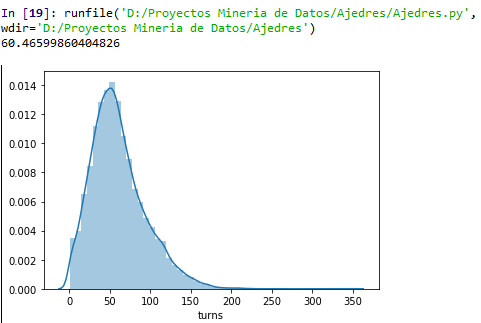
\includegraphics[width=0.27\textwidth]{ImagenesA/PruebaUno.png}
\caption{Grafica realizada con la libreria seaborn}
\end{figure}

\section{Prueba Dos(Análisis simple)}\\
Leemos el estado de la victoria, el cual sea igual a "Jaque mate" y sumamos el total de número de turnos de los juegos terminados en “mate”. Por medio de la librería .loc el cual nos permite realizar condiciones y acotar las respuestas, es decir buscar una resultado más cercano a lo que se desea encontrar.
\begin{figure}[h!]
\centering
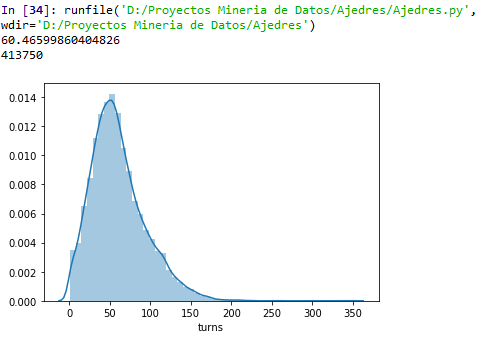
\includegraphics[width=0.27\textwidth]{ImagenesA/PruebaDos.png}
\caption{Grafica realizada con la libreria seaborn}
\end{figure}


\section{Conceptos}

\begin{itemize}
\item Exploración: \\
La exploración se basa en utilizar las técnicas de análisis en la exploración de datos, deducir la simetría, la distribución y la normalidad de los datos. Además de analizar las correlaciones que existen en la información (González, 2008, P.6).
\item Selección:\\  
La selección se basa en recopilar e integrar fuentes de datos existentes. También se basa en identificar y seleccionar las variables más relevantes en los datos. Además de aplicar técnicas de muestreo adecuadas (González, 2008, P.6).
\item Vista minable: \\
Vista minable se puede definir como la colección de individuos a los cuales queremos realizar un estudio, con todas sus respectivas características - atributos, con el fin de poder aplicar el proceso de minería sobre dichos datos y poder sustraer información útil (Alcober,Calduch y Zuñiga.2007).
\item Visualización:\\ 
Se basa en poder observar patrones, tendencias, anomalías para poder comprender los datos de una forma rápida.
La visualización se divide en posterior, previa y coordenadas paralelas:
Posterior: Se usa para validar y mostrar los resultados de la extracción. 
\begin{enumerate}
\item Previa: \\
Se usa para comprender de una mejor manera los datos y sugerir patrones.
Coordenadas 
\item paralelas: \\
Se usa para ingresar información en dimensiones que facilite su entendimiento, para poder detectar atributos, valores entre otros. 
(Manzanares,Chavez,Hernandez,Martinez,Alegria.2016).
\item Coordenadas paralelas: \\
Se usa para ingresar información en dimensiones que facilite su entendimiento, para poder detectar atributos, valores entre otros. 
(Manzanares,Chavez,Hernandez,Martinez,Alegria. 2016).
\end{enumerate}
\item Sumarización: \\
La sumarización permite observar los datos de una manera resumida, además de permitir el cálculo entre valores que no contienen datos directos. También permite realizar un análisis exploratorio de las partes (Manzanares,Chavez,Hernandez,Martinez,Alegria. 2016).
\item Generalización: \\ 
Una generalización busca resumir datos, reemplazando valores de un nivel relativamente bajo con conceptos de nivel alto o reduciendo el número de dimensiones para resumir los datos en el espacio conceptual (Han, Kamber, Pei.2011.P. 166). 
\item Pivotamiento: \\
También llamado rotar, es una operación de visualización que se basa en rotar los ejes de los datos con el fin de proporcionar una presentación de datos alterna  (Han, Kamber, Pei.2011.P. 148).
\end{itemize}

\section{Refencias}

\begin{itemize}
\item R.Alcover,J.,M.A.Calduch, L. R. Zúnica,(2007).Análisis del rendimiento académico en los estudios de informática de la Universidad Politécnica de Valencia aplicando técnicas de minería de datos.Universidad Politécnica de Valencia. 
Recuperado de: http://bioinfo.uib.es/~joemiro/aenui/procJenui/Jen2007/alanal.pdf
\item González D.(2008).Minería de Datos Técnicas y Herramientas.Recuperado el dia, 04,05,2019 de https://books.google.es/books?hl=es&lr=&id=wz-D_8uPFCEC&oi=fnd&pg=PR4&dq=que+es+exploracion+mineria+de+datos&ots=TiZ4zi4u7M&sig=BmOL29xv2Hye_LLDsIHdCeRXCkI#v=onepage&q=20exploracion20&f=.false.
\item Manzanares. J ,Chávez. A, Hernandez. J,Martinez. G,Alegria. J.(2016).Minería de Datos ( Exploración Y Selección).
Recuperado de: https://prezi.com/wz9-wj0ie9wz/mineria-de-datos-exploracion-y-seleccion/.
\item Han J, Kamber M, Pei J.(2011).Data Mining Concepts and Techniques .Recuperado el dia, 04,05,2019 de http://myweb.sabanciuniv.edu/rdehkharghani/files/2016/02/The-Morgan-Kaufmann-Series-in-Data-Management-Systems-Jiawei-Han-Micheline-Kamber-Jian-Pei-Data-Mining.-Concepts-and-Techniques-3rd-Edition-Morgan-Kaufmann-2011.pdf.


\end{itemize}
\ifCLASSOPTIONcaptionsoff
  \newpage
\fi




\end{document}
